%!TEX root = ../thesis_phd.tex
%%%%%%%%%%%%%%%%%%%%%%%%%%%%%%%%%%%%%%%%%%%%%%%%%%%%%%%%%%%%%%%%%%%%%%%%%%%%%%%%
% reconstruction.tex:
%%%%%%%%%%%%%%%%%%%%%%%%%%%%%%%%%%%%%%%%%%%%%%%%%%%%%%%%%%%%%%%%%%%%%%%%%%%%%%%%
\chapter{Event Reconstruction}
\label{reconstruction_chapter}
%%%%%%%%%%%%%%%%%%%%%%%%%%%%%%%%%%%%%%%%%%%%%%%%%%%%%%%%%%%%%%%%%%%%%%%%%%%%%%%%

In order to extract useful physics information from the \nova detector, the raw data (cell hits) must be processed into higher level forms.
This processing step is known as reconstruction.
For this analysis, the primary goals of reconstruction are to identify \numu charged-current (CC) interactions and estimate the energy of the neutrinos involved in the interactions. Identification of \numu CC interactions is really a task of rejecting backgrounds induced by both cosmic rays and the \numi beam.  The cosmic ray background dominantly composed of down-going muons, although other particles can also be present.  Backgrounds in the \numi beam include both neutral current (NC) interactions and CC interactions from \nue or \nutau.

Traditional reconstruction efforts involve detection of lines and other shapes in raw data.  Classification is then a process of extracting manually engineered features from those events which discriminate between signal and background.
This analysis uses machine learned features in a convolutional neural network to replace manual feature engineering.
In this approach, the hits themselves are presented to the neural network as two images, one each for both the $x$ (vertical) and $y$ horizontal plane views.
The goal with this approach is to sidestep pathological failures incurred in each reconstruction and feature engineering step, thus allowing more of those pathological events to be more correctly classified.

The \nova \textit{event display} provides a visualization of the raw detector readout which serves as the input to reconstruction.
An example event display is shown in figure \ref{eventDisplay14}.
The data corresponds to 550 $\mu s$ of Far Detector (FD) readout, with hits colored according to their time recorded relative to the start of the readout window.
Visible activity displayed falls into two primary groups: randomly distributed electronic noise and correlated activity from cosmic rays.
Since cosmic rays cross the detector quickly, hits along each track are displayed as a uniform color.

\begin{figure}[t]
\begin{center}
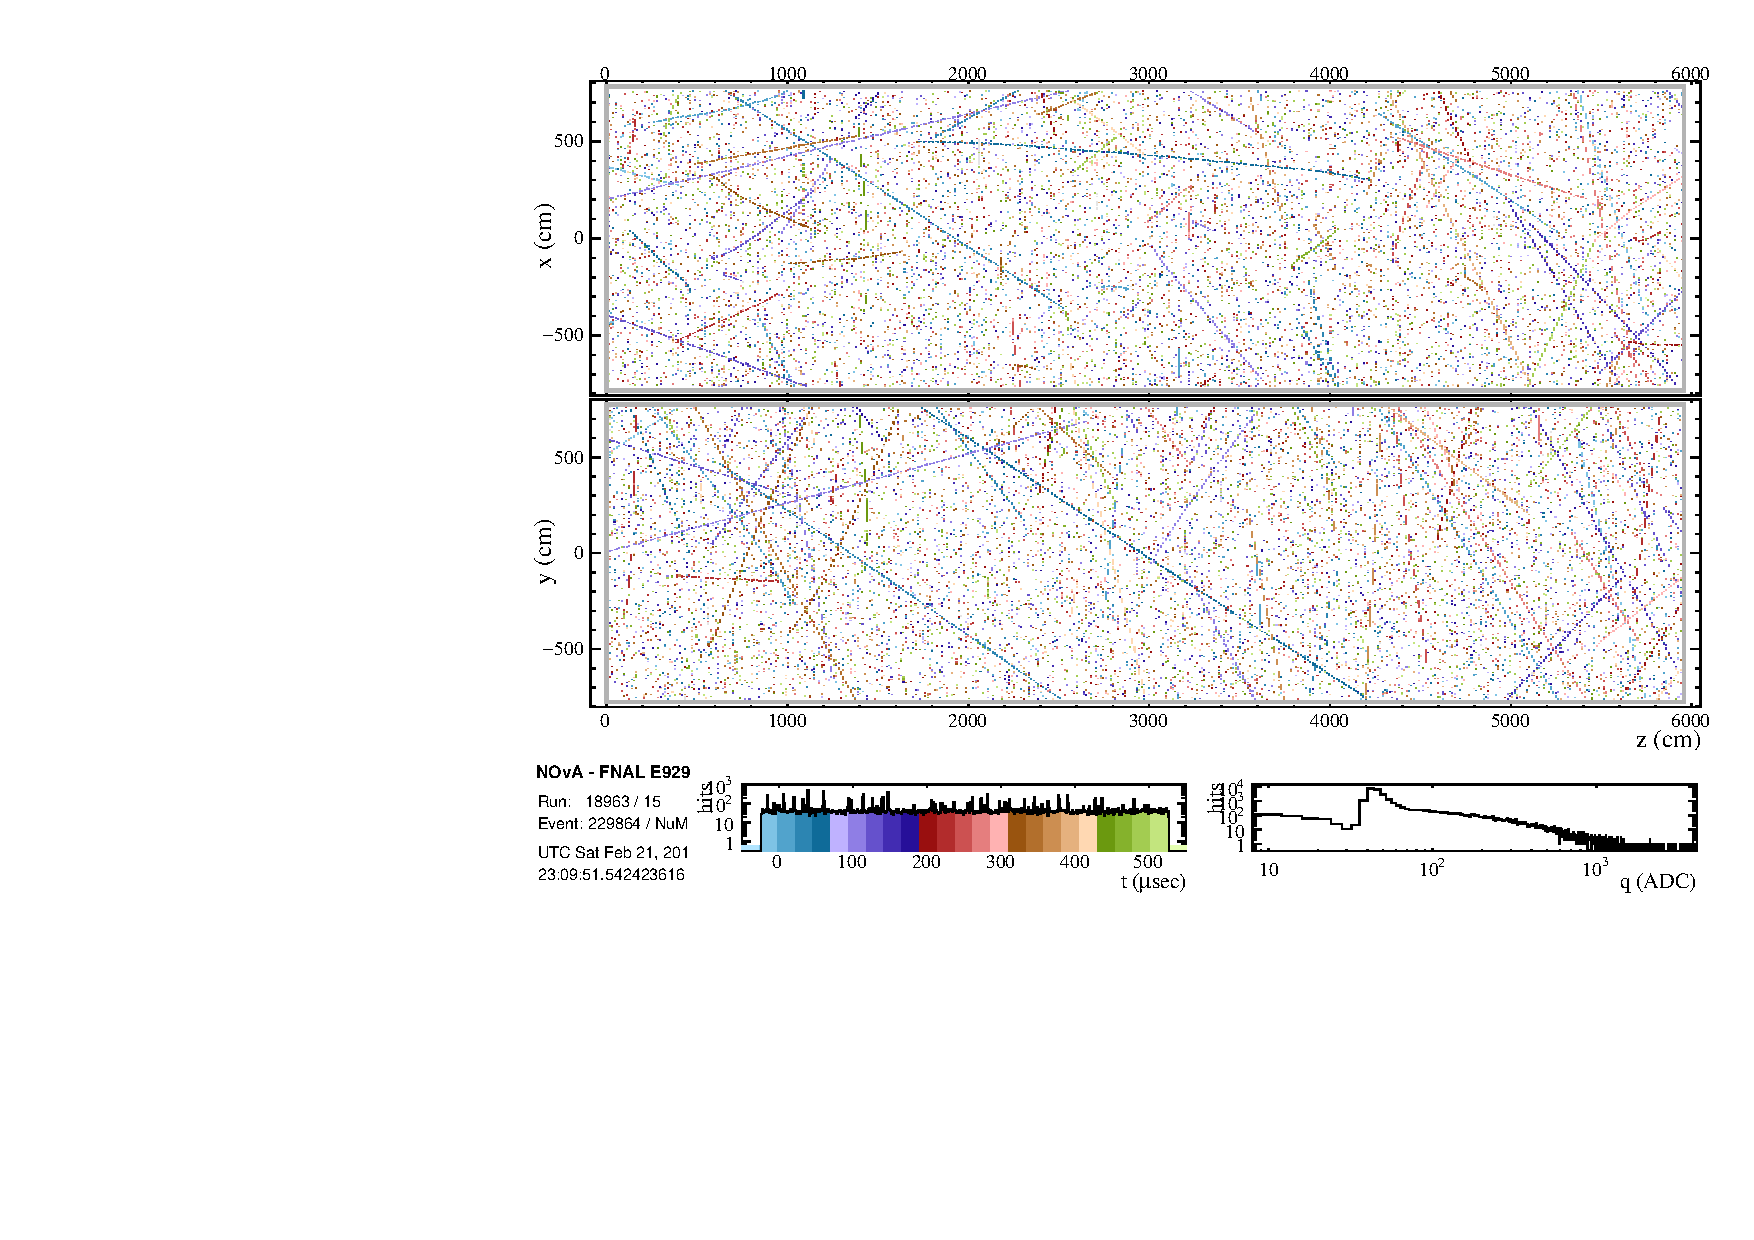
\includegraphics[width=\textwidth]{figures/evd/evd_14db.pdf}
\end{center}
\caption{An example \nova event display.  The top projection is an $x$ vs. $z$ view, the bottom is $y$ vs. $z$.  Hits are colored by the at which they were recorded relative to the start of the readout window; the color scale is visible in the bottom center pane.}
\label{eventDisplay14}
\end{figure}

\section{Slicing}

The first task in reconstructing \nova data is to resolve individual particle interactions


\section{Calibration}


\section{Image Formation}

\section{Architecture and Training}

We use siamese googlenet, two googlenets side-by-side

We train first for all event types



%%%%%%%%%%%%%%%%%%%%%%%%%%%%%%%%%%%%%%%%%%%%%%%%%%%%%%%%%%%%%%%%%%%%%%%%%%%%%%%%
